\section{Zusammenhang HTTP(s) und Zertifikate}
\label{sec:HTTPs}
Typischerweise fragt ein Nutzer eine Internetseite über das unsichere Hypertext Transfer Protocol (HTTP) an. Dabei werden alle benötigten Informationen wie zum Beispiel Benutzername und Passwort im Klartext übermittelt. Ebenfalls wird die Rückantwort unverschlüsselt übertragen. Für einen sicheren Datenaustausch sollte ein Anwender, falls dies angeboten wird, die Internetseite per Hypertext Transfer Protocol Secure (HTTPs) aufrufen. \cite[vgl.]{RFC7230} 
\\Seriöse Online-Banking-Webseiten unterstützen beispielsweise nur noch HTTPs-Aufrufe. Dabei wird dem Aufrufer durch das Kürzel HTTPs in der Adressleiste signalisiert, dass es sich hierbei um eine verschlüsselte Verbindung handelt. Genauer gesagt bedeutet es, dass eine HTTP-Kommunikation über SSL (Secure Sockets Layer) / TLS (Transport Layer Security) verschlüsselt abläuft. Bei jeder HTTPs-Kommunikation muss sich der Webserver, auf dem die Internetseite gehostet wird, gegenüber des Webseitenaufrufers, meist ein Client, authentifizieren. Für den Client besteht hierbei kein Muss, im Normalfall wird in der Praxis auf die clientseitige Authentifizierung verzichtet. Die Authentifizierung des Webservers gegenüber des Clients erfolgt durch ein für den Webserver ausgestelltes Zertifikat\footnote{Es handelt sich hierbei in der Regel um digitale Zertifikate nach dem ITU-T X.509 Standard \cite[vgl.]{RFC6101}}. \cite[vgl.]{RFC2818} 
Dieses enthält unter anderem den öffentlichen Schlüssel (Public Key), einen eindeutigen Fingerabdruck und Angaben über den Zertifikatsinhaber. \cite[vgl.]{x.509} Ein Zertifikat verbindet somit eindeutig einen Inhaber mit einem öffentlichen Schlüssel. Mit dem Public Key kann der Client verschiedene Daten, z. B. einen Pre-Shared Key, verschlüsselt zum Webserver schicken. Anhand des Fingerabdrucks, welcher auch als digitale Signatur des Zertifikats bezeichnet wird, überprüft der Client vor der Datenübermittlung, ob er mit dem richtigen Webserver kommuniziert. Der Fingerabdruck wird durch einen Hash-Algorithmus wie z. B. SHA-2 erzeugt. Bei der Erzeugung gehen diverse Informationen wie z. B. Zertifikatsaussteller, öffentlicher Schlüssel und Identifizierungsdaten über den Webserver mit ein. 
Wenn das Zertifikat von einer Zertifizierungsstelle (Certification Authority = CA) ausgestellt wurde, deren eigenes Zertifikat (= Root-Zertifikat oder Wurzelzertifikat) bereits im Browser installiert ist, dann wird dem ausgestellten Zertifikat automatisch vertraut. In den bekanntesten Webbrowsern wie z. B. Firefox, Chrome oder dem Internet Explorer sind bereits viele Root-Zertifikate von weltweit verschiedenen Zertifizierungsstellen vorinstalliert.
\begin{figure}[H]
		\centering
		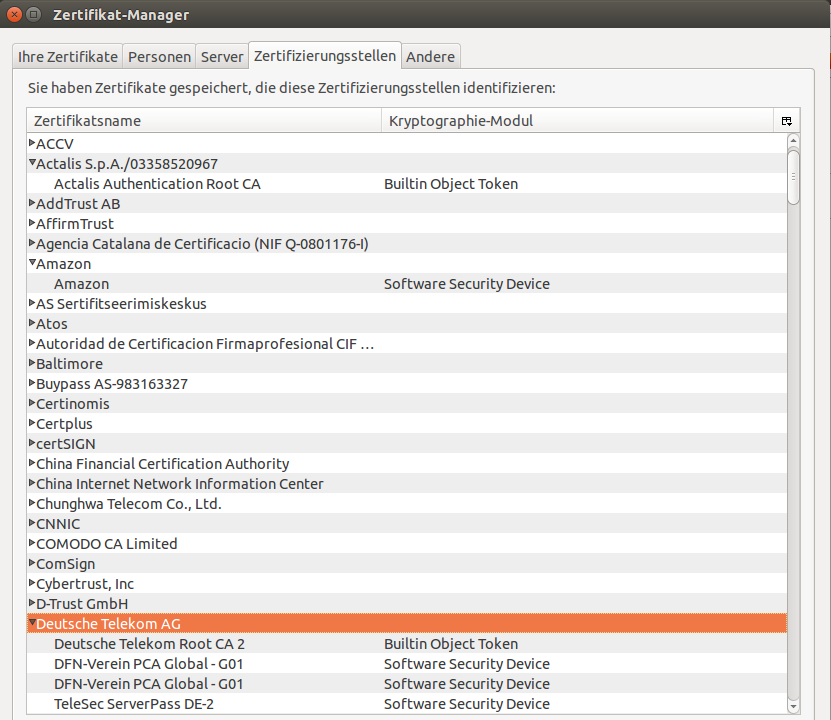
\includegraphics[width=0.5\linewidth]{images/Zertifizierungsstellen.png}
		\caption{Ausschnitt vorinstallierter Zertifizierungsstellen und deren ausgestellten Zertifikate im Firefox Browser}
\end{figure}
\noindent
Nutzt der Webservers ein selbst ausgestelltes (selbst signiertes) Zertifikat zur Authentifizierung, dann wird beim Verbindungsaufbau dem Nutzer eine Warnung angezeigt. Der Nutzer kann anschließend selbst entscheiden ob er dem Zertifikat vertraut oder nicht. Außerdem entscheidet er über Dauerhaftigkeit des Vertrauens, entweder nur ein einziges Mal, d. h. nur für diese Verbindungssession, oder für immer. 

\begin{figure}[htb]
	\centering
	\begin{minipage}[t]{0.65\linewidth}
	%	\centering
		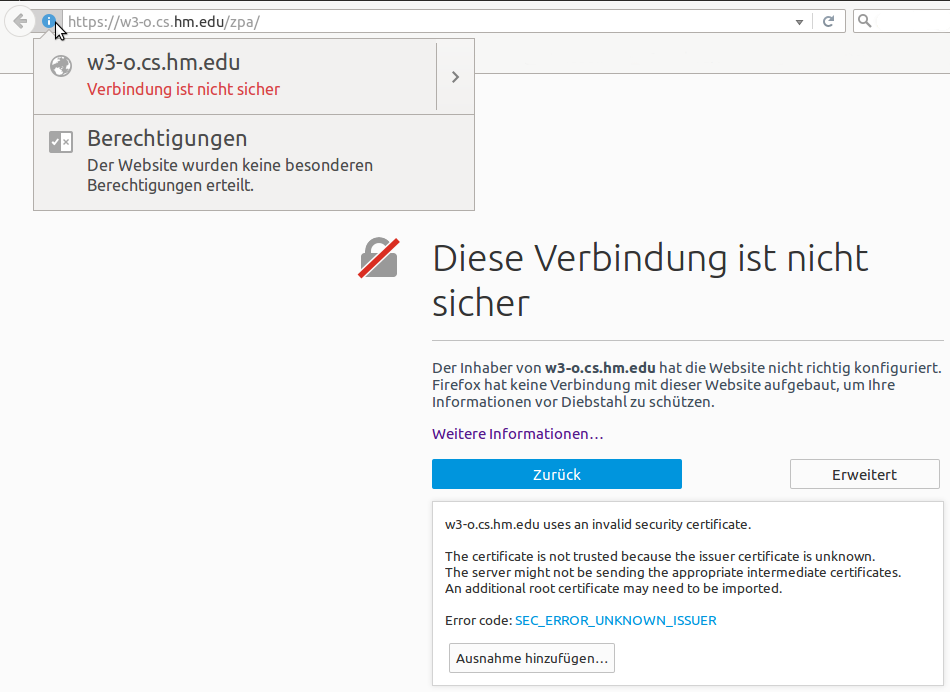
\includegraphics[width=.75\linewidth]{images/untrusted_ca.png}
		\caption{Warnung bei unbekanntem / \newline nicht vertrauenswürdigem Zertifikat}
	\end{minipage}% <- sonst wird hier ein Leerzeichen eingefügt
	\hfill
	\begin{minipage}[t]{0.35\linewidth}
		\centering
		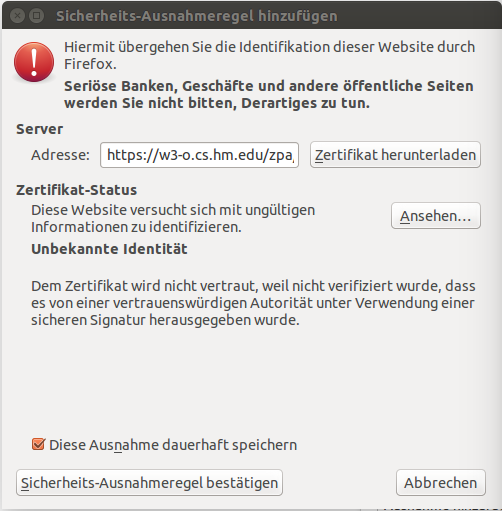
\includegraphics[width=\linewidth]{images/ausnahmeregel.png}
		\caption{Ausnahmeregel für ein unbekanntes / bislang nicht vertrauenswürdiges Zertifikat}
	\end{minipage}
\end{figure}

\noindent
Ist letzteres der Fall, dann wird das Zertifikat fest im Browser installiert. Es wird dann bei den schon vorinstallierten Zertifikaten mit abgelegt. Diese dauerhafte Ausnahme hat zu Folge, dass der Benutzer beim Verbindungsaufbau zu der zugehörigen Webseite vom Webbrowser nicht mehr gewarnt wird. 
\begin{figure}[H]
	\centering
	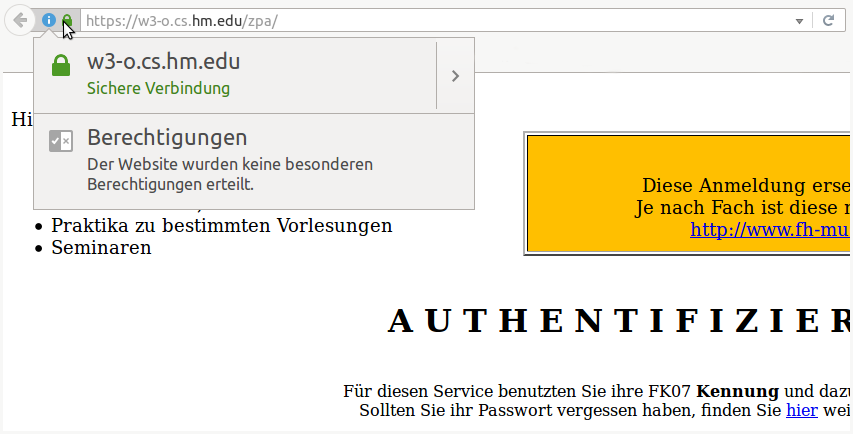
\includegraphics[width=.5\linewidth]{images/trusted_ca.png}
	\caption{Keine Warnung nach dauerhafter Ausnahme / fester Installation des Zertifikats im Browser}
\end{figure}